%%%%%%%%%%%%%%%%%%%%%%%%%%%%%%%%%%%%%%%%%
%
% (c) 2018 by Jennifer Laaser
%
% This work is licensed under the Creative Commons Attribution-NonCommercial-ShareAlike 4.0 International License. To view a copy of this license, visit http://creativecommons.org/licenses/by-nc-sa/4.0/ or send a letter to Creative Commons, PO Box 1866, Mountain View, CA 94042, USA.
%
% The current source for these materials is accessible on Github: https://github.com/jlaaser/quantum-exercises
%
%%%%%%%%%%%%%%%%%%%%%%%%%%%%%%%%%%%%%%%%%

%\documentclass[answers,addpoints,11pt]{exam}
\documentclass[addpoints,11pt]{exam}

\usepackage{amsmath}
\usepackage{braket}
\usepackage{listings}
\usepackage{graphicx}
%\usepackage{minipage}
\usepackage{array}
\usepackage{hyperref}
\usepackage{enumitem}


\newcolumntype{L}[1]{>{\raggedright\let\newline\\\arraybackslash\hspace{0pt}}m{#1}}
\newcolumntype{C}[1]{>{\centering\let\newline\\\arraybackslash\hspace{0pt}}m{#1}}
\newcolumntype{R}[1]{>{\raggedleft\let\newline\\\arraybackslash\hspace{0pt}}m{#1}}

\renewcommand{\sectionmark}[1]{\markboth{#1}{}}

\pagestyle{headandfoot}
\firstpageheadrule
\firstpagefootrule
\runningheadrule
\runningfootrule
\firstpageheader{}{\leftmark}{}
\runningheader{}{\leftmark}{}
\firstpagefooter{
\includegraphics[width=0.1\textwidth]{by-nc-sa} J. Laaser 2018}{}{Page \thepage\ of \numpages}
\runningfooter{
\includegraphics[width=0.1\textwidth]{by-nc-sa} J. Laaser 2018}{}{Page \thepage\ of \numpages}

\newcommand{\exptval}[1]{\left< #1 \right>}
\newcommand{\intallx}{\int_{-\infty}^{\infty}}
\newcommand{\adag}{\hat a^\dag}
\newcommand{\umat}[1]{\,\underline{\underline{#1}}}
\newcommand{\uvec}[1]{\,\underline{#1}}
\newcommand{\genpar}[3]{\frac{\partial^{#3}{#1}}{\partial {#2}^{#3}}}

\newcommand{\contdnewpg}{\begin{flushright}(Continued on back of page $\rightarrow$)	\end{flushright}\newpage }
%\newcommand{\pausenewpg}{\begin{flushright}(Pause here before going on $\rightarrow$)	\end{flushright}\newpage }
\newcommand{\answerbox}[1]{\raisebox{-2ex}{\framebox(#1,30){}}}
\newcommand{\answerboxtall}[1]{\raisebox{-4ex}{\framebox(#1,45){}}}


\author{Jennifer Laaser}
\title{In-Class Exercises for Quantum Chemistry}
\date{\today}

%% To output only one of the exercises, uncomment this line and replace the path with the path to the exercise you want to print:
%\includeonly{includes/states-funcs-vecs}

\begin{document}
	
%%%%%%%%%%%%%%%%%%%%%%%%%%%%%%%%%%%%%%%%%
%
% This work is licensed under the Creative Commons Attribution-NonCommercial-ShareAlike 4.0 International License. To view a copy of this license, visit http://creativecommons.org/licenses/by-nc-sa/4.0/ or send a letter to Creative Commons, PO Box 1866, Mountain View, CA 94042, USA.
%
% The current source for these materials is accessible on Github: https://github.com/jlaaser/quantum-exercises
%
%%%%%%%%%%%%%%%%%%%%%%%%%%%%%%%%%%%%%%%%%

\begin{titlepage}
\makeatletter
\centering

~

\vspace{1.5in}
{\LARGE \@title }
\vspace{0.5in}




\includegraphics[width=0.2\textwidth]{by-nc-sa}
\vspace{0.1in}

\begin{minipage}{0.75\textwidth}
\textcopyright 2018 by Jennifer Laaser. \@title\ is made available under a Creative Commons Attribution-NonCommercial-ShareAlike 4.0 International License: \url{http://creativecommons.org/licenses/by-nc-sa/4.0/}

\vspace{0.1in}

The current source for these materials is accessible on Github:\\ \url{https://github.com/jlaaser/quantum-exercises}
\end{minipage}


\vspace{0.5in}
Current revision: \@date

\end{titlepage}

\makeatother
\newpage
%%%%%%%%%%%%%%%%%%%%%%%%%%%%%%%%%%%%%%%%%%
%
% (c) 2018 by Jennifer Laaser
%
% This work is licensed under the Creative Commons Attribution-NonCommercial-ShareAlike 4.0 International License. To view a copy of this license, visit http://creativecommons.org/licenses/by-nc-sa/4.0/ or send a letter to Creative Commons, PO Box 1866, Mountain View, CA 94042, USA.
%
% The current source for these materials is accessible on Github: https://github.com/jlaaser/quantum-exercises
%
%%%%%%%%%%%%%%%%%%%%%%%%%%%%%%%%%%%%%%%%%

\section*{About the Exercises\sectionmark{About the Exercises}}

\clearpage

\begin{center}

~

\vspace{3in}
This page intentionally left blank.
\end{center}
%%%%%%%%%%%%%%%%%%%%%%%%%%%%%%%%%%%%%%%%%
%
% (c) 2018 by Jennifer Laaser
%
% This work is licensed under the Creative Commons Attribution-NonCommercial-ShareAlike 4.0 International License. To view a copy of this license, visit http://creativecommons.org/licenses/by-nc-sa/4.0/ or send a letter to Creative Commons, PO Box 1866, Mountain View, CA 94042, USA.
%
% The current source for these materials is accessible on Github: https://github.com/jlaaser/quantum-exercises
%
%%%%%%%%%%%%%%%%%%%%%%%%%%%%%%%%%%%%%%%%%

\section*{Quantum States: Analogies to Functions and Vectors\sectionmark{Exercise: States, Functions, \& Vectors}}

	Quantum states are abstract, but we can get some intuition for their properties by drawing analogies to functions and vectors.

	\begin{questions}
	
		\question Use your knowledge about functions and vectors to predict what expression should go in each of the blank cells in this table. A few of the lines are filled out to get you started.
		
			%\vspace{-0.2in}
			\begin{center}
				\renewcommand{\arraystretch}{1.5}
			\begin{tabular}{|C{2in}| C{2in} | C{2in}|}
				\hline
				
				\textbf{Functions} 
				& \textbf{Vectors}  
				& \textbf{Quantum States}
				\\
				\hline
				
				$f(x)$
				& $\vec v = \begin{pmatrix} v_1 \\ v_2 \\ v_3\end{pmatrix}$
				& $\ket{\alpha}$
				\\
				\hline
				
				$f^*(x)$
				& $\vec v\,^\dag = \begin{pmatrix} v_1^* & v_2^* & v_3^*\end{pmatrix}$
				& $\bra{\alpha}$
				\\
				\hline
				
				$h(x) = f(x) + g(x)$
				&
				& \vspace{0.75in}
				\\
				\hline
				
				& $\left( c\vec v \right)^\dag = c^* \vec v\,^\dag$
				& \vspace{0.75in}
				\\
				\hline
				
				$\int_{-\infty}^\infty dx\, f^*(x) f(x)$
				& $\vec v\,^\dag \vec v$
				& $\braket{\alpha|\alpha}$
				\\
				\hline
				
				&$\left(\vec u\,^\dag \vec v\right)^* = \vec v\,^\dag \vec u$
				& \vspace{0.75 in}
				\\
				\hline
				
				$\int_{-\infty}^\infty dx\, f^*(x) f(x) \geq 0$
				&
				& \vspace{0.75 in}
				\\
				\hline
				
				
			\end{tabular}
			\end{center}
		
		\emph{Note: we are using a very general notation here that allows vectors and functions to have complex values. If $\vec u$ and $\vec{v}$ are purely real, however, then $\vec u \,^\dag \vec v$ is just equal to the dot product $\vec u \cdot \vec v$ - I encourage you to try working through this if you are unsure about why it should be true.}
		
		\vspace{0.25in}
		\begin{flushright}(Continued on back of page $\rightarrow$)	\end{flushright}
		
		\newpage
		\question If $\vec a$ is a vector, then $\vec a\,^\dag \vec a$ gives the square of the length of the vector.
			\begin{parts}
				\part Why is it always true that $\vec a\,^\dag \vec a > 0$?
					\begin{solution}[1.5in]
					\end{solution}
				
				\part In this context, how would you interpret $\braket{\alpha|\alpha}$?
					\begin{solution}[1.5in]
					\end{solution}
			\end{parts}
		\question If $\vec a$ and $\vec b$ are vectors, then the \emph{projection} of $\vec{b}$ onto $\vec{a}$ is
			\begin{center}
			\begin{minipage}{0.4\textwidth}
					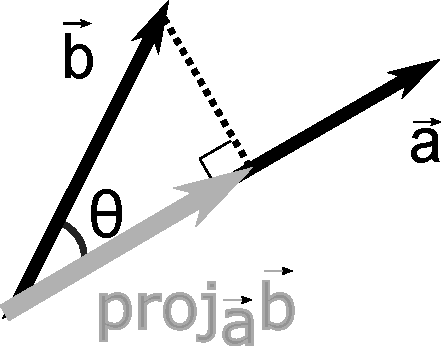
\includegraphics[width=0.7\textwidth]{includes/states-funcs-vecs-FIGURES/vector_projection.pdf}
			\end{minipage}
			\begin{minipage}{0.4\textwidth}
					\begin{align*}
						proj_{\vec a}\vec{b} &= \left(\text{length}\right)\left(\text{direction}\right) \\
						&= \left(|\vec{b}|cos(\theta)\right)\left( \frac{\vec{a}}{|\vec{a}|}\right) \\
							&= \left(|\vec{b}|\frac{\vec{a}\,^\dag\vec{b}}{|\vec{a}||\vec{b}|}\right)\left( \frac{\vec{a}}{|\vec{a}|}\right) \\
							&= \frac{\vec a\,^\dag \vec{b}}{|\vec{a}|^2}\vec{a} 
					\end{align*}
			\end{minipage}
			\end{center}
		
			\vspace{0.2in}
			In this context, how would you interpret the following expression? 
			\begin{equation*}		
				\frac{\braket{\alpha|\beta}}{\braket{\alpha|\alpha}}\ket{\alpha}
			\end{equation*}

	\end{questions}


%%%%%%%%%%%%%%%%%%%%%%%%%%%%%%%%%%%%%%%%%
%
% (c) 2018 by Jennifer Laaser
%
% This work is licensed under the Creative Commons Attribution-NonCommercial-ShareAlike 4.0 International License. To view a copy of this license, visit http://creativecommons.org/licenses/by-nc-sa/4.0/ or send a letter to Creative Commons, PO Box 1866, Mountain View, CA 94042, USA.
%
% The current source for these materials is accessible on Github: https://github.com/jlaaser/quantum-exercises
%
%%%%%%%%%%%%%%%%%%%%%%%%%%%%%%%%%%%%%%%%%

\section*{Understanding Operators\sectionmark{Understanding Operators}}

	In this exercise, you will again use functions as a model for understanding some of the properties of operators.
	(You will do a similar exercise with vectors on your first problem set.)

	\begin{questions}
	
		\question $\hat A$ and $\hat B$ are operators that each operate on a function (left column) to give a new function (right column).
			\vspace{0.2in}
			
			\centerline{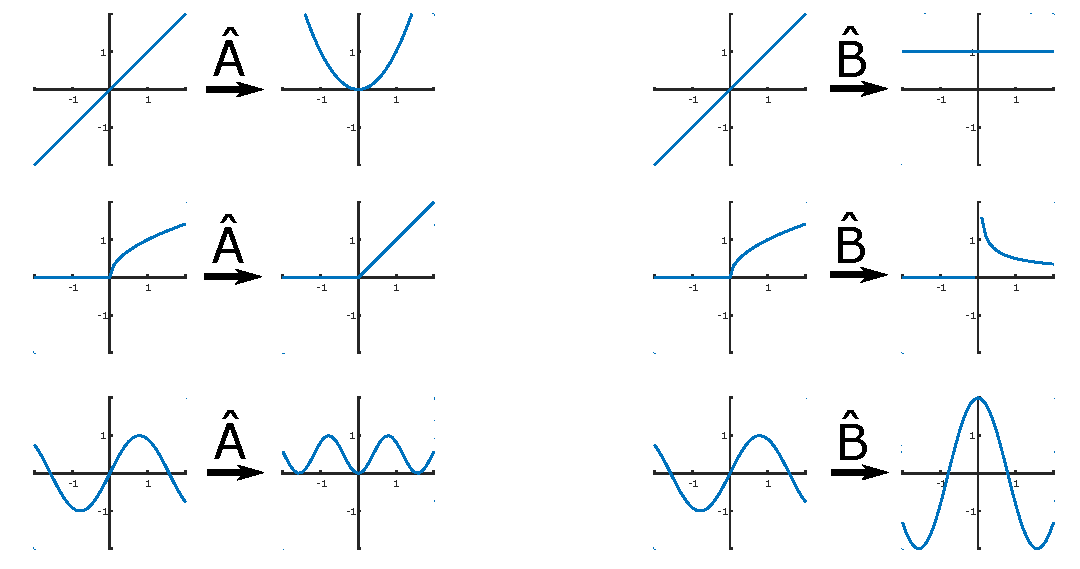
\includegraphics[width=\textwidth]{includes/operators-FIGURES/functions_operators}}
			\vspace{0.2in}
		
			\begin{parts}
			
				\part Describe, in words, what each operator does to a function.
				
					\begin{solution}[2.3in]
					\end{solution}
				
				\part Fill in the blanks by writing mathematical forms for each operator:
				
					\begin{align*}
						\hat A f(x) =  \raisebox{-2ex}{\framebox(60,30){}} & & \hat B f(x) =  \raisebox{-2ex}{\framebox(60,30){}}				
					\end{align*}
				
				\begin{flushright}(Continued on back of page $\rightarrow$)	\end{flushright}
				\part Predict what functions would result from the following operations:
				
		\vspace{0.2in}	\centerline{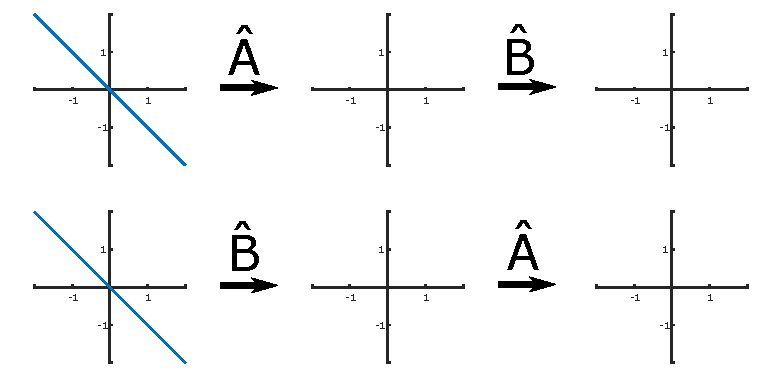
\includegraphics[width=0.7\textwidth]{includes/operators-FIGURES/functions_commutation.pdf}}
			
				\vspace{0.2in}
				
				If the function on the left is $f(x)$, then one of the plots on the right corresponds to $\hat A \hat B f(x)$ and one corresponds to $\hat B \hat A f(x)$.  Circle the plot that you think corresponds to $\hat A \hat B f(x)$.
				
					\vspace{0.2in}
				
				\part From your results, do you think $\hat A \hat B \ket{\Psi}$ will usually be equal to $\hat B \hat A  \ket{\Psi}$?  Why or why not?
				
					\begin{solution}[2in]
					\end{solution}
				
				\part Are there any functions $f(x)$ and $g(x)$ for which $\hat A f(x) = f(x)$ and $\hat B g(x) = g(x)$?  If so, what are they?
			\end{parts}	
	
	\end{questions}


%%%%%%%%%%%%%%%%%%%%%%%%%%%%%%%%%%%%%%%%%
%
% (c) 2018 by Jennifer Laaser
%
% This work is licensed under the Creative Commons Attribution-NonCommercial-ShareAlike 4.0 International License. To view a copy of this license, visit http://creativecommons.org/licenses/by-nc-sa/4.0/ or send a letter to Creative Commons, PO Box 1866, Mountain View, CA 94042, USA.
%
% The current source for these materials is accessible on Github: https://github.com/jlaaser/quantum-exercises
%
%%%%%%%%%%%%%%%%%%%%%%%%%%%%%%%%%%%%%%%%%

\section*{Eigenfunctions and Eigenvalues\sectionmark{Eigenfunctions and Eigenvalues}}

	\begin{questions}
		\question Assume $\ket{f}$ is an eigenket of $\hat\Omega$ with eigenvalue $\omega$, i.e.
			\begin{equation*}
				\hat\Omega \ket{f} = \omega\ket{f}
			\end{equation*}
			
			\begin{parts}
			
				\part What is $\braket{f|\hat\Omega|f}$?
					\begin{solution}[1in]
					\end{solution}
					
				\part What is $\braket{f|\hat\Omega|f}^*$?
					\begin{solution}[1in]
					\end{solution}
					
				\part If $\hat \Omega$ is Hermitian, then your answers to the preceding two parts have to be equal.  
				
					What does that tell you about the values of $\omega$ and $\omega^*$?
				
					\begin{solution}[1.5in]
					\end{solution}
					
				\part If a number is equal to its complex conjugate, then can the number have a non-zero imaginary part? Why or why not?
				
					\begin{solution}[1.5in]
					\end{solution}
					
				\part What does that tell you about the value of $\omega$?
				
					\begin{solution}[1in]
					\end{solution}
			\begin{flushright}(Continued on back of page $\rightarrow$)	\end{flushright}
					
			\end{parts}
			
		\newpage
		\question The Kronecker delta, $\delta_{ij}$, equals 1 when $i=j$ and is 0 when $i\neq j$.
		
			\begin{parts}
				\part Write out the first few terms of the sum $\sum_j \delta_{3j} c_j$.  What does it simplify to?
				
					\begin{solution}[1in]
					\end{solution}
			
				\part More generally, what do you think $\sum_j \delta_{ij} c_j$ will simplify to?
				
					\begin{solution}[1in]
					\end{solution}
				
			\end{parts}
			
		\question We can always choose the eigenstates $\{\ket{i}\}$ of a Hermitian operator such that the overlap of an eigenstate with itself equals 1 and the overlap of an eigenstate with a different eigenstate equals 0, i.e. such that
			\begin{equation*}
				\braket{i|j} = \delta_{ij}
			\end{equation*}
			
			\begin{parts}
				\part If we write $\ket{\Psi}$ as a linear combination of these eigenstates, i.e.
					\begin{equation*}
						\ket{\Psi} = \sum_j c_j\ket{j}
					\end{equation*}
					what is $\braket{i|\Psi}$?
				
					\begin{solution}[2in]
					\end{solution}
					
				\part Substitute your answer back into $\ket{\Psi} = \sum_j c_j\ket{j}$.
				
					Why might we say that $\sum_i \ket{i}\bra{i}$ is just equivalent to multiplying by 1?
			\end{parts}
			
	\end{questions}


%%%%%%%%%%%%%%%%%%%%%%%%%%%%%%%%%%%%%%%%%
%
% (c) 2018 by Jennifer Laaser
%
% This work is licensed under the Creative Commons Attribution-NonCommercial-ShareAlike 4.0 International License. To view a copy of this license, visit http://creativecommons.org/licenses/by-nc-sa/4.0/ or send a letter to Creative Commons, PO Box 1866, Mountain View, CA 94042, USA.
%
% The current source for these materials is accessible on Github: https://github.com/jlaaser/quantum-exercises
%
%%%%%%%%%%%%%%%%%%%%%%%%%%%%%%%%%%%%%%%%%

\section*{Wavefunctions and Probabilities\sectionmark{Wavefunctions and Probabilities}}
	
	If $\ket{\Psi} = \sum_i c_i \ket{i}$, where the $\{\ket{i}\}$ are the eigenstates of operator $\hat\Omega$, then
	\begin{align*}
		\braket{\Psi|\hat\Omega|\Psi} &= \left(\sum_i c_i^* \bra{i}\right) \hat\Omega \left(\sum_j c_j \ket{j}\right)\\
			&= \sum_i |c_i|^2 \omega_i
	\end{align*}
	(You will prove this on your first homework set.)
	
	\begin{questions}
	
		\question This has a similar form to a weighted average, e.g.
			\begin{equation*}
				\left\langle \omega \right\rangle = \sum_i P_i \omega_i
			\end{equation*}
			where $P_i$ is the probability of measuring value $\omega_i$. 
			In this context, how would you interpret $|c_i|^2$?
			
			\begin{solution}[1in]
			\end{solution}
			
		\question Remember that you can find $c_i$ by calculating $\braket{i|\Psi}$. Given this, how would you interpret the value of $\left|\braket{i|\Psi}\right|^2$?
			
			\begin{solution}[1in]
			\end{solution}
		
		\question A particularly useful set of eigenstates are the eigenstates of the position operator, $\hat x$, where eigenstate $\ket{x_1}$ corresponds to the eigenstate in which we measure the position of the particle as being exactly at $x=x_1$ and nowhere else.
		
			In this context, how would you interpret the value of $|\braket{x_1|\Psi}|^2$?
			
			\begin{solution}[1.75in]
			\end{solution}
			\begin{flushright}(Continued on back of page $\rightarrow$)	\end{flushright}
		
		\newpage
		\question More generally, how would you interpret the function $|\Psi(x)|^2$ where $\Psi(x) = \braket{x|\Psi}$?
		
			\begin{solution}[2in]
			\end{solution}
			
		\question What should have to be true about the value of $\int_{-\infty}^{\infty} dx\, |\Psi(x)|^2$?
		
			\emph{Hint: what should the total probability of finding the particle \emph{somewhere} along the x axis be?}
		
			\begin{solution}
			\end{solution}
		
	\end{questions}
	

%%%%%%%%%%%%%%%%%%%%%%%%%%%%%%%%%%%%%%%%%
%
% (c) 2018 by Jennifer Laaser
%
% This work is licensed under the Creative Commons Attribution-NonCommercial-ShareAlike 4.0 International License. To view a copy of this license, visit http://creativecommons.org/licenses/by-nc-sa/4.0/ or send a letter to Creative Commons, PO Box 1866, Mountain View, CA 94042, USA.
%
% The current source for these materials is accessible on Github: https://github.com/jlaaser/quantum-exercises
%
%%%%%%%%%%%%%%%%%%%%%%%%%%%%%%%%%%%%%%%%%

\section*{Time-Evolution of the Wavefunction\sectionmark{Exercise: Time Evolution}}

	We can describe the time-evolution of a quantum state $\ket{\Psi}$ using the time-evolution operator $\hat U (t)$, which relates the state of the system at time $t=t_1$ to the state of the system at time $t=0$ by
	\begin{equation*}
		\ket{\Psi(t=t_1)} = \hat U(t_1) \ket{\Psi(t=0)}
	\end{equation*}
	$\hat U(t)$ is given by 
	\begin{equation*}
		\hat U(t) = e^{-i\hat H t/\hbar}
	\end{equation*}
	where $\hat H$ is the Hamiltonian operator corresponding to the total energy of the system.
	
	\begin{questions}
	
		\vspace{0.2in}
		\question If $\ket{n}$ is an eigenstate of $\hat H$, then
			\begin{equation*}
				\hat H\ket{n} = E_n\ket{n}
			\end{equation*}	
			where $E_n$ is the total energy of a system in eigenstate $\ket{n}$.
			
			Using this information, fill in the blanks for the following expressions:
			
			\begin{align*}
				\hat H^2\ket{n} = \hat H \left(\hat H \ket{n}\right) =  \raisebox{-2ex}{\framebox(60,30){}} & & \hat H^3 \ket{n} =   \raisebox{-2ex}{\framebox(60,30){}} & & \hat H^i \ket{n} =  \raisebox{-2ex}{\framebox(60,30){}}
			\end{align*}
			
			\vspace{0.1in}
		\question Applying $\hat U(t)$ directly to $\ket{n}$ is tricky because $\hat H$ is in the exponent. However, we can do it if we use the Taylor-series expansion $e^x \approx 1 + x + \frac{1}{2!} x^2 + ...$.
		
			Fill in the blanks in the following derivation:
			
			\begin{align*}
				\hat U(t)\ket{n} &= e^{-i\hat H t/\hbar}\ket{n}\\
				&= \left(1 + \raisebox{-2ex}{\framebox(40,40){}} + \frac{1}{2!}\raisebox{-2ex}{\framebox(40,40){}}  + ...\right)\ket{n}\\
				&= \left( \ket{n} + \left(\frac{-it}{\hbar}\right)\hat H^{\framebox(20,20){}}\ket{n} + \frac{1}{2!} \left(\frac{-it}{\hbar}\right)^2\hat H^{\framebox(20,20){}}\ket{n} + ...\right)\\
				&= \left( \ket{n} + \left(\frac{-it}{\hbar}\right) E_n^{\framebox(20,20){}}\ket{n} + \frac{1}{2!} \left(\frac{-it}{\hbar}\right)^2 E_n^{\framebox(20,20){}}\ket{n} + ...\right)\\
				&= \left(1 + \raisebox{-2ex}{\framebox(40,40){}} + \frac{1}{2!}\raisebox{-2ex}{\framebox(40,40){}}  + ...\right)\ket{n}\\
				&= e^{-i E_n t/\hbar}\ket{n}
			\end{align*}
			
			\vspace{0.2in}
			\begin{flushright}(Continued on back of page $\rightarrow$)	\end{flushright}
		
		\newpage
		\question If we express $\ket{\Psi(t=0)}$ as a linear combination of energy eigenstates, e.g.
			\begin{equation*}
				\ket{\Psi(t=0)} = \sum_n c_n \ket{n}
			\end{equation*}
			then how would you find $\ket{\Psi(t=t_1)}$?
			
			\emph{(Hint: start by substituting this expression into $\ket{\Psi(t=t_1)} = \hat U(t_1)\ket{\Psi(t=0)}$, and note that you can move $\hat U(t_1)$ through the sum since it is a linear operator.)}
	
	\end{questions}
%%%%%%%%%%%%%%%%%%%%%%%%%%%%%%%%%%%%%%%%%
%
% (c) 2018 by Jennifer Laaser
%
% This work is licensed under the Creative Commons Attribution-NonCommercial-ShareAlike 4.0 International License. To view a copy of this license, visit http://creativecommons.org/licenses/by-nc-sa/4.0/ or send a letter to Creative Commons, PO Box 1866, Mountain View, CA 94042, USA.
%
% The current source for these materials is accessible on Github: https://github.com/jlaaser/quantum-exercises
%
%%%%%%%%%%%%%%%%%%%%%%%%%%%%%%%%%%%%%%%%%

\section*{Position and Momentum: Eigenfunctions and Operators\sectionmark{Exercise: Position and Momentum}}

	Two particularly useful operators in quantum mechanics are the position operator, $\hat x$, and the momentum operator, $\hat p$.
	
	In this set of exercises, we will consider what these operators and their eigenfunctions look like in the position representation.
	
	\vspace{0.25in}
	
	\begin{questions}
		\question An eigenstate of the position operator is one where the probability of finding the particle is nonzero at only one position.
		
			\begin{parts}
				\part Predict what the probability density for a particle found at $x=x_0$ should look like:
				
\vspace{0.5in}					\centerline{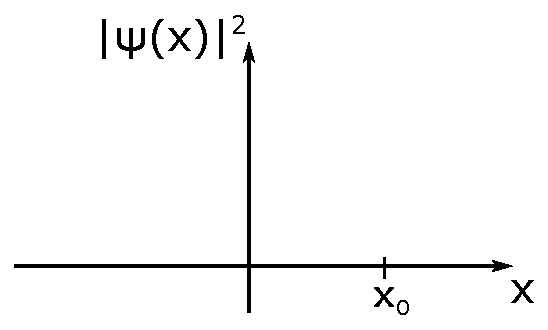
\includegraphics[width=0.5\textwidth]{includes/xp-eigenfuns-eigenvals-FIGURES/x0_axes}}		
\vspace{0.3in}		
				
				\part The eigenvalue of this position eigenstate should be the particle's position, e.g. $x_0$. Which of the following operators would be most useful for extracting this eigenvalue?
				
				\begin{align*}
					\hat \Omega \psi(x) &= \psi(x) + x  && (\hat\Omega = \text{``add x'')}\\
					\hat \Omega \psi(x) &= x\psi(x)&& (\hat\Omega = \text{``multiply by x'')}\\
					\hat \Omega \psi(x) &= |\psi(x)|^2&& (\hat\Omega = \text{``square the function'')}\\
					\hat \Omega \psi(x) &= \frac{d}{dx}\psi(x)  && (\hat\Omega = \text{``take the derivative'')}
				\end{align*}
				
				Briefly explain your choice:
				
				\begin{solution}[1.5in]
				\end{solution}
			
			\end{parts}
			
			
		\begin{flushright}(Continued on back of page $\rightarrow$)	\end{flushright}
		\newpage 
		\item De Broglie told us that a particle with momentum $p$ has wavelength $\lambda = \frac{h}{p}$.
		
			\begin{parts}
				\part One useful function that has a wave-like form is $f(x) = e^{ikx} = \cos(kx) + i\sin(kx)$.  What is the wavelength of this function in terms of $k$ (i.e. for what value of $\lambda$ does $f(x+\lambda) = f(x)$)?
				
					\begin{solution}[2in]
					\end{solution}
				
				\part Set this wavelength equal to de Broglie's value for $\lambda$. How is $k$ related to $p$?
				
					\begin{solution}[2in]
					\end{solution}
				
				
				\part What operator might you be able to apply to the function $e^{ikx}$ to extract the momentum eigenvalue $p$?
				
					\begin{solution}[2in]
					\end{solution}
				
			\end{parts}
	\end{questions}
\section*{The Particle in a Box\sectionmark{The Particle in a Box}}

	\begin{questions}
	
		\question Consider a particle in the following one-dimensional ``particle in a box'' potential:
		
			\vspace{0.1in}
			\centerline{
				\begin{minipage}{0.5\textwidth}
					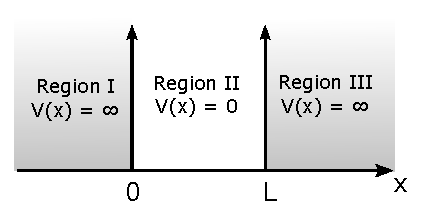
\includegraphics[width=\textwidth]{includes/PIB-FIGURES/PIB}
				\end{minipage}
				\begin{minipage}{0.3\textwidth}
					\begin{equation}
				 		V(x)=\begin{cases}\infty & x<0 \\ 0 & 0 \leq x \leq L \\ \infty & x>L \end{cases} \nonumber
					\end{equation}
				\end{minipage}
		}\vspace{0.1in}
		
			\begin{parts}
			
				\part What is the Hamiltonian in Region II, where $V(x) = 0$?
				
					\begin{equation*}
						\hat H = \answerbox{75}
					\end{equation*}
				
				\part Show that $\Psi(x) = A\cos(kx) + B\sin(kx)$ is an eigenfunction of this Hamiltonian $\hat H$.  What is its eigenvalue?
				
					\begin{solution}[2.75in]
					\end{solution}
				
				\part Set this eigenvalue equal to the energy, $E$. What is $E$ in terms of $k$?
				
					\begin{solution}[1.75in]
					\end{solution}
					
			\end{parts}
			
			\contdnewpg 
			
			\question
				\begin{parts}
			
				\part It is physically impossible for the particle to be in the regions where $V(x) = \infty$, so the probability of finding the particle in these regions has to be zero. 
				
				What does this tell you about the value of the wavefunction in Regions I and III?
					\begin{align*}
						\Psi_{I}(x) = \answerbox{40} & & \Psi_{III}(x) = \answerbox{40}
					\end{align*}
				
				\part The wavefunction must be continuous at every value of $x$.  What does that mean must be true about the value of $\Psi_{II}(x)$ at the edges of the box?
					\begin{align*}
						\Psi_{II}(0) = \answerbox{40} & & \Psi_{II}(L) = \answerbox{40}
					\end{align*}
					
				\part Using the wavefunction $\Psi_{II}(x) = A\cos(kx) + B\sin(kx)$, calculate $\Psi_{II}(0)$ and set it equal to the value you found above. What does this tell you about the value of $A$?
				
					\begin{solution}[2in]
					\end{solution}
				
				\part Now, calculate $\Psi_{II}(L)$. What has to be true about $kL$ in order for $\Psi_{II}(L)$ to equal what you found in part (b)? What does this result tell you about the values of the energy $E$?
				
					\begin{solution}[1.75in]
					\end{solution}
		
			\end{parts}
	\end{questions}


\section*{The Free Particle\sectionmark{The Free Particle}}

Suppose a particle is traveling in a constant one-dimensional potential, $V(x)=V_c$.
	\begin{questions}
		\question What is the Hamiltonian for this particle?
				
					\begin{equation*}
						\hat H = \answerbox{75}
					\end{equation*}
					\vspace{0.1in}
				
		\question What is the Schr\"odinger equation for this particle?
					
					\begin{solution}[1.75in]
					\end{solution}
				
		\question Try a solution of the form $\Psi(x) = e^{sx}$. What is $s$ in terms of the potential $V_c$, the particle's energy $E$, and the particle's mass, $m$?
					
					\begin{solution}[4.25in]
					\end{solution}
				
				\contdnewpg 
					
		\question If the particle's energy is greater than the potential, e.g. $E>V_c$, is $s$ real or imaginary?  Sketch the shape of the resulting wavefunction on the graph below:
		
			\vspace{0.45in}
			\centerline{
				\begin{minipage}{0.5\textwidth}
				.
				\end{minipage}
				\begin{minipage}{0.4\textwidth}
					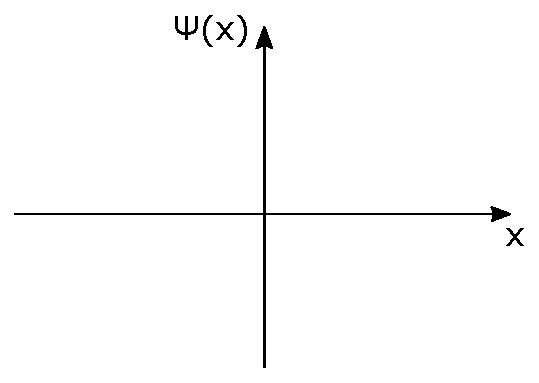
\includegraphics[width=\textwidth]{includes/free-particle-FIGURES/psi_axes.pdf}
				\end{minipage}
			}
			\vspace{0.45in}
				
		\question If the particle's energy is less than the potential, e.g. $E<V_c$, is $s$ real or imaginary?  Sketch the shape of the resulting wavefunction on the graph below:
		
			\vspace{0.45in}
			\centerline{
				\begin{minipage}{0.5\textwidth}
				.
				\end{minipage}
				\begin{minipage}{0.4\textwidth}
					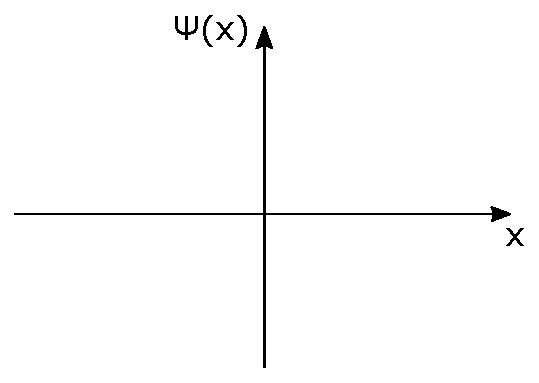
\includegraphics[width=\textwidth]{includes/free-particle-FIGURES/psi_axes.pdf}
				\end{minipage}
			}
			\vspace{0.45in}
				
		\question Why are the wavefunctions you found in questions 4 and 5 difficult to normalize?
	\end{questions}
	

%%%%%%%%%%%%%%%%%%%%%%%%%%%%%%%%%%%%%%%%%
%
% (c) 2018 by Jennifer Laaser
%
% This work is licensed under the Creative Commons Attribution-NonCommercial-ShareAlike 4.0 International License. To view a copy of this license, visit http://creativecommons.org/licenses/by-nc-sa/4.0/ or send a letter to Creative Commons, PO Box 1866, Mountain View, CA 94042, USA.
%
% The current source for these materials is accessible on Github: https://github.com/jlaaser/quantum-exercises
%
%%%%%%%%%%%%%%%%%%%%%%%%%%%%%%%%%%%%%%%%%

\section*{Tunneling\sectionmark{Tunneling}}

	Consider a particle incident ``from the left'' on the following potential barrier, with the particle's energy less than the barrier height, e.g. $E<V_0$:
		
			\vspace{0.1in}
			\centerline{
				\begin{minipage}{0.5\textwidth}
					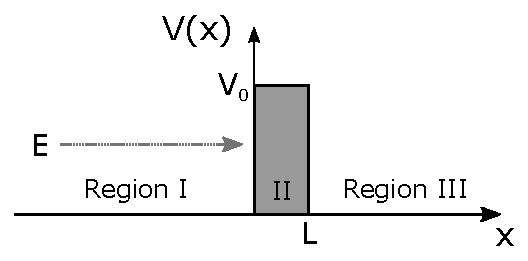
\includegraphics[width=\textwidth]{includes/tunneling-FIGURES/tunneling.pdf}
				\end{minipage}
				\begin{minipage}{0.3\textwidth}
					\begin{equation}
				 		V(x)=\begin{cases}0 & x<0 \\ V_0 & 0 \leq x \leq L \\ 0 & x>L \end{cases} \nonumber
					\end{equation}
				\end{minipage}
		}\vspace{-0.1in}

	\begin{questions}
	
		\question What are the general solutions for the wavefunction in each region? Make sure to include any appropriate coefficients.
		
			\begin{minipage}{0.1\textwidth}.
			\end{minipage}
			\begin{minipage}{0.4\textwidth}
			\begingroup
\addtolength{\jot}{1em}
			\begin{align*}
				\Psi_I(x) = \answerbox{150}\\
				\Psi_{II}(x) = \answerbox{150}\\
				\Psi_{III}(x) = \answerbox{150}
			\end{align*}
			\endgroup
			\end{minipage}
			\begin{minipage}{0.4\textwidth}
			\begingroup
\addtolength{\jot}{1em}
			\begin{align*}
				k = \answerboxtall{60}\\
				\kappa = \answerboxtall{60}
			\end{align*}
			\endgroup
			\end{minipage}
			
			\vspace{0.1in}
		\question What are the boundary conditions necessary for...
		
			\begin{parts}
				\part ... the \emph{wavefunction} to be continuous at $x=0$ and $x=L$?
				
					%\emph{(Note: you don't need to plug anything into the wavefunctions; it's sufficient to write your answers in the form of $\Psi_I(x_0) = \Psi_{II}(x_0)$, etc.)}
				
					\begin{solution}[1.5in]
					\end{solution}
				
				\part ... the \emph{first derivative} of the wavefunction  to be continuous at $x=0$ and $x=L$?
				
					\begin{solution}[1.3in]
					\end{solution}
				
				\contdnewpg 
				
				\part ... the particle to be incident only from the left?
				
					\begin{solution}[1.5in]
					\end{solution}
				
				%\part ... ``arbitrary'' normalization?
				
				%	\begin{solution}[1.5in]
				%	\end{solution}
			\end{parts}
		
		\question What ratio would you calculate if you wanted to find the probability that the particle is transmitted through the barrier (e.g. the tunneling probability)?
				
					\begin{solution}[1.5in]
					\end{solution}
		
		\question If you do all the algebra, you will find that the tunneling probability for a tall, thin barrier is approximately
			\begin{equation*}
				T = \frac{16E(V_0-E)}{V_0^2} e^{-2\sqrt{\frac{2m(V_0-E)}{\hbar^2}}L}
			\end{equation*}
			
			What do you predict would happen to to the tunneling probability if...
			\begin{parts}
				\part ... you increased the particle's mass?
				
					\begin{solution}[1.5in]
					\end{solution}
				
				\part ... you decreased the barrier width?
				
					\begin{solution}[1.5in]
					\end{solution}
			\end{parts}
	\end{questions}	
	
%%%%%%%%%%%%%%%%%%%%%%%%%%%%%%%%%%%%%%%%%
%
% (c) 2018 by Jennifer Laaser
%
% This work is licensed under the Creative Commons Attribution-NonCommercial-ShareAlike 4.0 International License. To view a copy of this license, visit http://creativecommons.org/licenses/by-nc-sa/4.0/ or send a letter to Creative Commons, PO Box 1866, Mountain View, CA 94042, USA.
%
% The current source for these materials is accessible on Github: https://github.com/jlaaser/quantum-exercises
%
%%%%%%%%%%%%%%%%%%%%%%%%%%%%%%%%%%%%%%%%%

\section*{Wavepackets\sectionmark{Exercise: Wavepackets}}

\begin{questions}
\question Activity time!  Get everyone in your group to stand up and stand shoulder-to-shoulder in a straight line.  You may go out in the hallway if you need more room.

	\begin{parts}
		\part Have everyone walk forward for 5 seconds.  Try to walk at as close to the same speed as possible.  Mark each person's initial and final positions on the following axis:

	\vspace{0.2in}
	\centerline{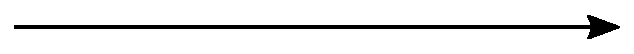
\includegraphics[width=0.6\textwidth]{includes/wavepackets-FIGURES/long-arrow.pdf}}
	\vspace{0.2in} 
		
		\part Go back to your starting line.  Have everyone walk forward for 5 seconds again, but this time, designate at least one person as a ``fast'' walker and one as a ``slow'' walker.  Mark each person's initial and final positions on the following axis:

	\vspace{0.2in}
	\centerline{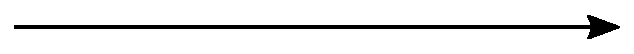
\includegraphics[width=0.6\textwidth]{includes/wavepackets-FIGURES/long-arrow.pdf}}
	\vspace{0.2in} 
		
		\part In which of these two ``simulations'' was the uncertainty in your momentum higher?  How was it reflected in your final position distribution?
			\begin{solution}[1.5in]
			\end{solution}
	\end{parts}

\question Consider a Gaussian wavepacket traveling to the right. At $t=0$, its probability distribution might look like this:

	\vspace{0.1in}
	\centerline{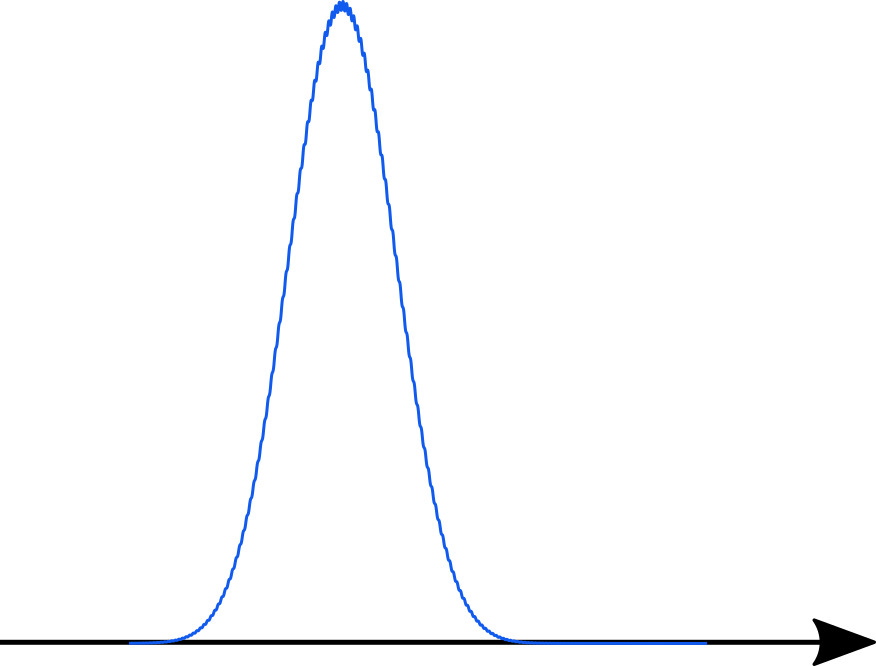
\includegraphics[width=0.35\textwidth]{includes/wavepackets-FIGURES/gaussian.jpg}}
	\vspace{0.1in} 
 
	\begin{parts}
		\part Based on the simulation you just did, what feature of this plot (if any) do you think gives you information about the uncertainty in the particle's position? Mark it on the plot.

		\part Similarly, what feature of this plot (if any) gives you information about the uncertainty in the particle's momentum?  Mark it on the plot.
	\end{parts}
	
	\contdnewpg

\question The following plots show the propagation of two different wavepackets:

      	\vspace{0.2in}
	\begin{minipage}{0.5\textwidth}
	\centerline{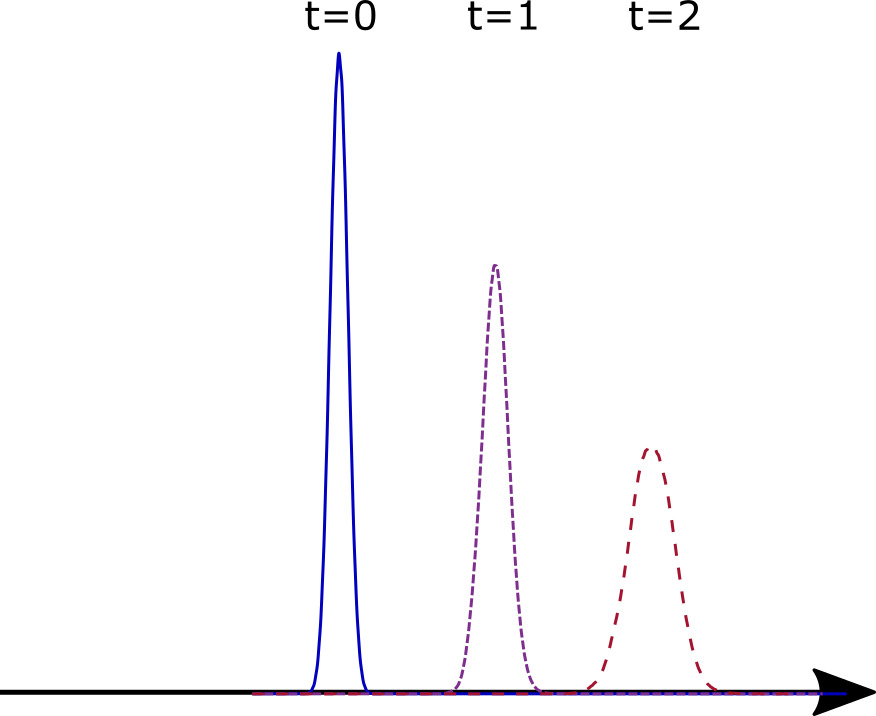
\includegraphics[width=0.8\textwidth]{includes/wavepackets-FIGURES/prop1.jpg}}
	\end{minipage}
	\begin{minipage}{0.5\textwidth}
	\centerline{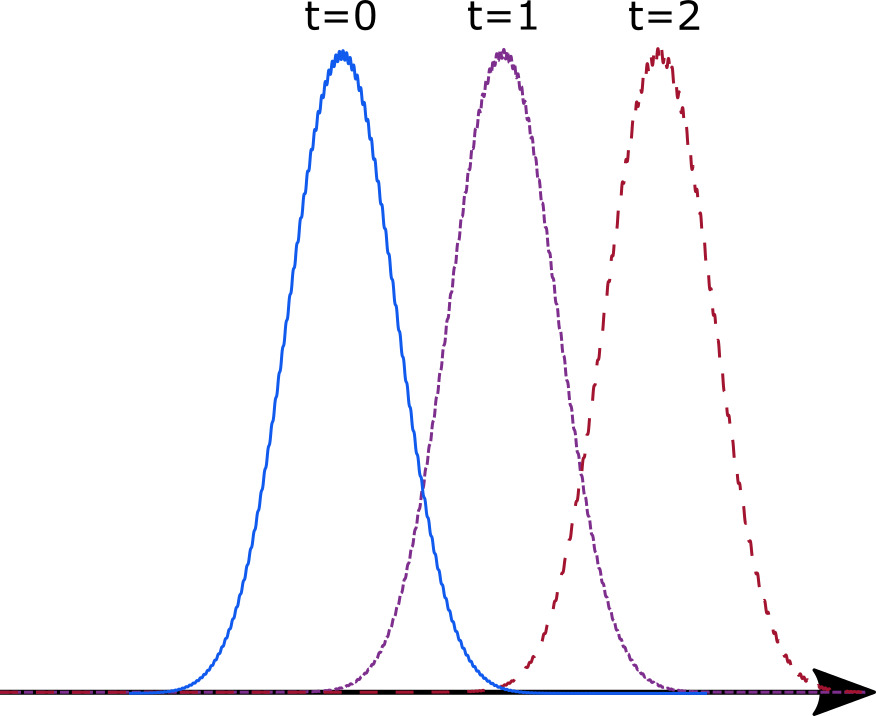
\includegraphics[width=0.8\textwidth]{includes/wavepackets-FIGURES/prop2.jpg}}
	\end{minipage}
	\vspace{0.1in}

\begin{parts}
\part Which wavepacket has the larger uncertainty in the position, and which has the larger uncertainty in the momentum?

	\begin{solution}[1.5in]
	\end{solution}

\part Explain how your observations relate to the uncertainty principle.
\end{parts}
	
	\begin{solution}[3.5in]
	\end{solution}

\end{questions}

\stophere
%%%%%%%%%%%%%%%%%%%%%%%%%%%%%%%%%%%%%%%%%
%
% (c) 2018 by Jennifer Laaser
%
% This work is licensed under the Creative Commons Attribution-NonCommercial-ShareAlike 4.0 International License. To view a copy of this license, visit http://creativecommons.org/licenses/by-nc-sa/4.0/ or send a letter to Creative Commons, PO Box 1866, Mountain View, CA 94042, USA.
%
% The current source for these materials is accessible on Github: https://github.com/jlaaser/quantum-exercises
%
%%%%%%%%%%%%%%%%%%%%%%%%%%%%%%%%%%%%%%%%%

\section*{Generalizing the Free Particle\sectionmark{Exercise: Generalizing the Free Particle}}

	In this set of exercises, we will explore how to think about an arbitrary wavefunction on a constant potential in terms of the free particle momentum eigenstates.

	\begin{questions}
	
		\question Let's start by considering how the wavefunction in the position representation is related to the wavefunction in the momentum representation.
		
			\begin{parts}
				\part The wavefunction in the position representation is given by $\Psi(x) = \braket{x\underset{\uparrow}|\Psi}$.
		
					Insert a complete set of momentum eigenstates at the arrow and simplify to find an expression for $\Psi(x)$ in terms of $\Psi(k)$.
		
				\begin{solution}[2.5in]
				\end{solution}
				
				\part Use the same process to find an expression for $\Psi(k) = \braket{k|\Psi}$ in terms of $\Psi(x)$.
				
					\begin{solution}[2.5in]
					\end{solution}
					
				\part Do you notice anything interesting about these relationships? If you know the formal name for this type of transformation, go ahead and write it down:
			
			\end{parts}
		\vspace{1in}
		\contdnewpg
		\question Now, let's consider the time-dependence of a particle on a constant potential.
		
			\begin{parts}
				\part If a system starts in a pure momentum eigenstate, i.e. $\Psi(x,t=0) = \phi_k(x)$, what is its \emph{time-dependent} wavefunction $\Psi(x,t)$?
				
					\emph{You'll probably find it useful to remember that on a constant potential $V(x)=0$, the momentum eigenstate with quantum number $k$ has wavefunction $\phi_k(x) = e^{ikx}$ and energy $E_k = \frac{\hbar^2 k^2}{2m}$.}
					
					\begin{solution}[3in]
					\end{solution}
			
				\part For a discrete set of eigenstates, a particle with $\Psi(x,t=0) = \sum_n c_n \phi_n(x)$ has time-dependent wavefunction $\Psi(x,t) = \sum_n c_n e^{-iE_nt/\hbar} \phi_n(x)$.
				
					By analogy, what do you think the time-dependent wavefunction should be for a particle with $\Psi(x,t=0) = \int_{-\infty}^{\infty} dk\, c(k) \phi_k(x)$?
				
			\end{parts}
	\end{questions}
	

%%%%%%%%%%%%%%%%%%%%%%%%%%%%%%%%%%%%%%%%%
%
% (c) 2018 by Jennifer Laaser
%
% This work is licensed under the Creative Commons Attribution-NonCommercial-ShareAlike 4.0 International License. To view a copy of this license, visit http://creativecommons.org/licenses/by-nc-sa/4.0/ or send a letter to Creative Commons, PO Box 1866, Mountain View, CA 94042, USA.
%
% The current source for these materials is accessible on Github: https://github.com/jlaaser/quantum-exercises
%
%%%%%%%%%%%%%%%%%%%%%%%%%%%%%%%%%%%%%%%%%

\section*{A Few Special Operators\sectionmark{Exercise: Harmonic Oscillator Operators}}

	In this set of exercises, we will look at the raising and lowering operators and their effect on eigenstates of the harmonic oscillator.

	\begin{questions}
	
		\question We showed that we can write the dimensionless Hamiltonian for the harmonic oscillator as 
			\begin{equation*}
				\hat h = \adag \hat a + \frac{1}{2}
			\end{equation*}
			This is just an operator ($\hat N = \adag \hat a$) plus a constant ($c = \frac{1}{2}$).
			
			\begin{parts}
				\part Suppose $\ket{n}$ is an eigenstate of $\hat N$ with eigenvalue $n$, i.e. $\hat N \ket{n} = n\ket{n}$. Is $\ket{n}$ also an eigenstate of $\hat h$?
				
					\begin{solution}[2.5in]
					\end{solution}
				
				\part How are the eigenvalues of $\ket{n}$ under $\hat N$ and $\hat h$ related?
				
					\begin{solution}[1.5in]
					\end{solution}
				
				\part Why does this mean we can solve the harmonic oscillator simply by finding the eigenstates of $\adag \hat a$?
				
					\begin{solution}[1.75in]
					\end{solution}
				
			\end{parts}

		\contdnewpg
		\question Now, let's consider what eigenvalue we would get from $\hat N$ if our starting state were $\hat a \ket{n}$.  We can write
			\begin{align*}
				\hat N(\hat a \ket{n}) &= (\adag \hat a)\hat a \ket{n} && \text{use definition of $\hat N$} \\
				 &= (\hat a \adag - 1)\hat a \ket{n} && \text{use }[\hat a,\adag] = 1 \\
				 &= (\hat a \adag \hat a - \hat a)\ket{n} && \text{distribute}\\
				 &= \hat a(\adag \hat a - 1)\ket{n} && \text{``reverse'' distribute}\\
				 &= \hat a(\hat N - 1)\ket{n} && \text{use definition of $\hat N$}\\
				 &= \hat a (n-1) \ket{n} && \text{use $\hat N \ket{n} = n\ket{n}$}\\
				 &= (n-1)(\hat a \ket{n})
			\end{align*}
			\begin{parts}
				\part Explain why this means $\hat a \ket{n}$ is also an eigenstate of $\hat N$.  What is its eigenvalue?
				
					\begin{solution}[2in]
					\end{solution}
				
				\part Explain why this might let us write $\hat a \ket{n} = c_n \ket{n-1}$.
				
					\begin{solution}[2in]
					\end{solution}
					
				\part Why might we call $\hat a$ a ``lowering'' operator?
				
					\begin{solution}[1.5in]
					\end{solution}
				
			\end{parts}
			
		\contdnewpg
		\question Now, we need to find the coefficient $c_n$.
		
			\begin{parts}
				\part If $\ket{n}$ is normalized, then what is $\braket{n|\hat N|n}$?
				
					\begin{solution}[2in]
					\end{solution}
				
				\part $\braket{n|\hat N|n}$ can also be written as $\braket{n|\adag \hat a|n}$.
				
					If $\hat a \ket{n} = c_n \ket{n-1}$, then $\bra{n}\adag = c_n^* \bra{n-1}$. Using this fact, and remembering that $\hat N = \adag \hat a$, calculate $\braket{n|\hat N|n}$ in terms of $c_n$.
				
					\begin{solution}[3in]
					\end{solution}
					
				\part Set your answers to the preceding two parts equal to each other. Solve for $c_n$, and fill in the blank in the following expression:
					\begin{equation*}
						\hat a \ket{n} = \answerbox{30}\ket{n-1}
					\end{equation*}
			\end{parts}
	\end{questions}
	

%%%%%%%%%%%%%%%%%%%%%%%%%%%%%%%%%%%%%%%%%
%
% (c) 2018 by Jennifer Laaser
%
% This work is licensed under the Creative Commons Attribution-NonCommercial-ShareAlike 4.0 International License. To view a copy of this license, visit http://creativecommons.org/licenses/by-nc-sa/4.0/ or send a letter to Creative Commons, PO Box 1866, Mountain View, CA 94042, USA.
%
% The current source for these materials is accessible on Github: https://github.com/jlaaser/quantum-exercises
%
%%%%%%%%%%%%%%%%%%%%%%%%%%%%%%%%%%%%%%%%%

\section*{Eigenvalues and Eigenstates of the Harmonic Oscillator\sectionmark{Exercise: Harmonic Oscillator Eigenstates}}

	\begin{questions}
		\question Let's start by considering the range of values that $n$ can take.
			\begin{parts}
				\part We know that for a quantum state $\alpha$, $\braket{\alpha|\alpha}\geq 0$.  What does this tell you about the minimum possible value of $\braket{n|\adag \hat a|n}$?
			
				\emph{(Hint: start by defining $\ket\alpha = \hat a\ket n$. What is $\bra{\alpha}$, and what do you get if you put these pieces together?)}
			
				\begin{solution}[3in]
				\end{solution}
			
				\part We also showed on the previous page that $\braket{n|\adag \hat a|n} = n$.  What does this tell you about the minimum possible value of $n$?
				
				\begin{solution}[1.5in]
				\end{solution}
				
				\part What happens if you try to calculate $\hat a \ket{0.5}$?  What do you think that means about whether $\ket{0.5}$ is an allowable quantum state for the harmonic oscillator?
				
					\begin{solution}[1.75in]
					\end{solution}
				\contdnewpg
				
				\part What happens if you calculate $\hat a \ket{1.5}$?  Given your answer to part (c), what do you think this means about whether $\ket{1.5}$ is an allowable quantum state?
				
					\begin{solution}[2in]
					\end{solution}
				
				\part Explain why this reasoning suggests that integers are the only allowable quantum numbers for the harmonic oscillator.
				
					\begin{solution}[3in]
					\end{solution}
			
			\end{parts}
			
		\question Suppose we knew what the eigenstate $\ket{0}$ was.  What might you do to find eigenstate $\ket{1}$?  How about $\ket{2}$, or $\ket{3}$?  How about $\ket{n}$?
		
			%\part Suppose we knew a functional form for $\braket{\xi|0} = \phi_0(\xi)$.  What might you do to find $\phi_1(\xi)$?
			
			\begin{solution}[2in]
			\end{solution}
			
	\end{questions}
	
	\stophere
%%%%%%%%%%%%%%%%%%%%%%%%%%%%%%%%%%%%%%%%%
%
% (c) 2018 by Jennifer Laaser
%
% This work is licensed under the Creative Commons Attribution-NonCommercial-ShareAlike 4.0 International License. To view a copy of this license, visit http://creativecommons.org/licenses/by-nc-sa/4.0/ or send a letter to Creative Commons, PO Box 1866, Mountain View, CA 94042, USA.
%
% The current source for these materials is accessible on Github: https://github.com/jlaaser/quantum-exercises
%
%%%%%%%%%%%%%%%%%%%%%%%%%%%%%%%%%%%%%%%%%

\section*{Describing States and Operators with Matrices\sectionmark{Exercise: Intro to Matrix Mechanics}}

	In this set of exercises, we will look at how vectors and matrices can be used to describe and calculate useful properties of quantum states and operators.

	\begin{questions}
	
		\question
		\begin{parts}
			\part Calculate the following matrix product:
			\begin{equation}
				\begin{bmatrix} c_1^* & c_2^* \end{bmatrix}
				\begin{bmatrix} A_{11} & A_{12} \\ A_{21} & A_{22} \end{bmatrix}
				\begin{bmatrix} c_1 \\ c_2 \end{bmatrix} \nonumber
			\end{equation}
			
				\begin{solution}[2.5in]
				\end{solution}
			
			\part Calculate $\exptval{A}=\braket{\psi|\hat A|\psi}$ where $\ket{\psi} = c_1 \ket{1} + c_2 \ket{2}$
			
				\begin{solution}[2.5in]
				\end{solution}
			
			\part Given your answers to the previous two questions, why might we call $\braket{n|\hat A|m}$ a ``matrix element'' of $\hat A$?
			
				\begin{solution}[1.3in]
				\end{solution}
			
			\contdnewpg
		\end{parts}
			
		\question 
		\begin{parts}
			\part If we calculate matrix elements of $\hat A$ using one basis set (e.g. the particle-in-a-box eigenstates), will it be the same as if we use a different basis set (e.g. the harmonic oscillator eigenstates)?  Why or why not?
			
				\begin{solution}[2.5in]
				\end{solution}
				
			\part Determine whether or not the following statement is correct, and briefly explain why or why not: ``If $\ket\Psi = \sum_n c_n \ket{n}$, and we clearly state what basis states the $\{\ket{n}\}$ represent, then the only thing we need to fully describe $\ket\Psi$ are the coefficients $c_n$.''
			
				\begin{solution}[2.5in]
				\end{solution}
				
			\part Write an analogous statement about how we might be able to describe $\hat A$ solely in terms of its matrix elements.
			
				\begin{solution}[2in]
				\end{solution}
		\end{parts}
		
		%	\question If the matrix element $A_{nm} = \braket{n|\hat A|m}$, and $\hat A$ is Hermitian, then what is $A_{mn}$?
		
		%		\begin{solution}[2.5in]
		%		\end{solution}
	\end{questions}
	
\stophere
%%%%%%%%%%%%%%%%%%%%%%%%%%%%%%%%%%%%%%%%%
%
% (c) 2018 by Jennifer Laaser
%
% This work is licensed under the Creative Commons Attribution-NonCommercial-ShareAlike 4.0 International License. To view a copy of this license, visit http://creativecommons.org/licenses/by-nc-sa/4.0/ or send a letter to Creative Commons, PO Box 1866, Mountain View, CA 94042, USA.
%
% The current source for these materials is accessible on Github: https://github.com/jlaaser/quantum-exercises
%
%%%%%%%%%%%%%%%%%%%%%%%%%%%%%%%%%%%%%%%%%

\section*{Eigenvalues, Eigenstates, and Eigenvectors\sectionmark{Eigenstates in Matrix Mechanics}}

	In this set of exercises, we will think about how to express eigenvalue-eigenstate relationships using the matrix formalism.
	
	\begin{questions}
		\question 
		\begin{parts}
			\part Using matrix notation, what needs to be true if $\ket\Psi = \sum_n c_n\ket n$ is an eigenstate of $\hat\Omega$ with eigenvalue $\omega$?
		
				\emph{Hint: in Dirac notation, we need $\hat\Omega \ket\Psi = \omega\ket\Psi$. What are the matrix-notation ``equivalents'' of $\hat\Omega$ and $\ket\Psi$?}
			
				\begin{solution}[2in]
				\end{solution}
			
			\part Using your answer to the preceding question, fill in the blank to complete the following statement:
			
				``If $\ket\Psi$ is an eigenstate of $\hat\Omega$, then the vector $\uvec{c} = \begin{pmatrix}c_1 \\ c_2 \\ c_3 \\ \vdots\end{pmatrix}$ must be an $\answerbox{120}$ of the matrix $\umat\Omega$.''
				
					\vspace{0.25in}
			
			\part Suppose we had a matrix $\umat\Omega$ containing the matrix elements of $\hat\Omega$ in some basis $\{\ket n\}$.
			
				Describe, in words, what steps you might take to find the vector $\uvec{c}$ that describes the eigenstate $\ket\Psi$ in terms of the $\{\ket n\}$ basis.
				
				\begin{solution}[2.6in]
				\end{solution}
				
				\contdnewpg
			
		\end{parts}
		
		\question Often, it is useful to be able to ``transform'' the matrix corresponding to an operator (most often the Hamiltonian) from one basis set to another.
		
			\begin{parts}
				\part Suppose the $\{\ket n\}$ are the true eigenstates of $\hat H$, such that $\hat H\ket n = E_n \ket n$.  Using Dirac notation, what are the matrix elements of $\hat H$ in this basis, i.e. what is $H_{nm}$?
				
					\begin{solution}[1.25in]
					\end{solution}	
				
				\part Now, assume we only know the matrix elements of $\hat H$ in some other basis, $\{\ket i\}$.  What are the matrix elements in this basis (i.e. what is $H_{ij}$?
				
					\begin{solution}[1.25in]
					\end{solution}	
				
				\part Take your expression from part (b) and insert a complete set of $\{\ket n\}$ eigenstates at each ``$|$'' (remember to use different indices - $n$ for the first set of eigenstates and $m$ for the second!).  What does this tell you about how you might be able to use matrix multiplication to ``transform'' $\umat H$ from one basis to another?
			\end{parts}
	\end{questions}

%%%%%%%%%%%%%%%%%%%%%%%%%%%%%%%%%%%%%%%%%
%
% (c) 2018 by Jennifer Laaser
%
% This work is licensed under the Creative Commons Attribution-NonCommercial-ShareAlike 4.0 International License. To view a copy of this license, visit http://creativecommons.org/licenses/by-nc-sa/4.0/ or send a letter to Creative Commons, PO Box 1866, Mountain View, CA 94042, USA.
%
% The current source for these materials is accessible on Github: https://github.com/jlaaser/quantum-exercises
%
%%%%%%%%%%%%%%%%%%%%%%%%%%%%%%%%%%%%%%%%%

\section*{Some Properties of the Angular Momentum Operators\sectionmark{Exercise: Commutation of Angular Momentum Operators}}

	In this set of exercises, we will look at commutation relationships of the angular momentum operators.  For this set of exercises, you'll find it useful to remember that the operator forms of $L_x$, $L_y$, and $L_z$ are given by
			\begin{align*}
				\hat L_x = \hat y \hat p_z - \hat z \hat p_y & &
				\hat L_y = \hat z \hat p_x - \hat x \hat p_z & &
				\hat L_z = \hat x \hat p_y - \hat y \hat p_x
			\end{align*}

	\begin{questions}
	
		\question If we calculate the commutator between $\hat L_x$ and $\hat L_y$, we find
			\begin{align*}
				[\hat L_x, \hat L_y] &= [\hat y \hat p_z-\hat z \hat p_y , \hat z \hat p_x - \hat x \hat p_z] \\
					&= [\hat y \hat p_z, \hat z \hat p_x] - [\hat y \hat p_z, \hat x \hat p_z] - [\hat z \hat p_y, \hat z \hat p_x] + [\hat z \hat p_y, \hat x \hat p_z]
			\end{align*}
			\begin{parts}
				\part Two of the commutators in the last line go to zero.  Which ones are they, and why are they zero?
				
					\begin{solution}[1.5in]
					\end{solution}
				
				\part The remaining two commutators simplify to $-i\hbar \hat y \hat p_x$ and $i\hbar \hat x \hat p_y$.  Which one is which?  Can you justify why they have these values?
				
					\begin{solution}[1.5in]
					\end{solution}
				
				\part Combine your answers to the previous two parts to find an expression for $[\hat L_x,\hat L_y]$. Your result will be proportional to either $\hat L_x$, $\hat L_y$, or $\hat L_z$ - which one is it, and what is the proportionality constant?
				
					\begin{solution}[1.5in]
					\end{solution}
			\end{parts}

		\contdnewpg
		
		We can generalize the results from the previous page to yield
		\begin{align*}
			[\hat L_x, \hat L_y] = i\hbar \hat L_z & & [\hat L_y, \hat L_z] = i\hbar \hat L_x & & [\hat L_z, \hat L_x] = i\hbar \hat L_y
		\end{align*}
		
		\question 
		
			\begin{parts}
				\part Can we measure two different components of the angular momentum simultaneously or not?
				
					\begin{solution}[1.5in]
					\end{solution}
			
				\part  The \emph{square magnitude} of the angular momentum is given by $\hat L^2 = \hat L_x^2 + \hat L_y^2 + \hat L_z^2$. Do $\hat L^2$ and $\hat L_z$ commute?
				
					\emph{You'll find it useful to remember that $[\hat A^2,\hat B] = \hat A[\hat A, \hat B] + [\hat A, \hat B]\hat A$}
				
					\begin{solution}[3.5in]
					\end{solution}
				
				\part Based on your result from part (b), can we measure the magnitude of the angular momentum and at least one of its components simultaneously or not?
				
					\begin{solution}[1.25in]
					\end{solution}
			\end{parts}
		
	\end{questions}
	
	
\stophere
%%%%%%%%%%%%%%%%%%%%%%%%%%%%%%%%%%%%%%%%%
%
% (c) 2018 by Jennifer Laaser
%
% This work is licensed under the Creative Commons Attribution-NonCommercial-ShareAlike 4.0 International License. To view a copy of this license, visit http://creativecommons.org/licenses/by-nc-sa/4.0/ or send a letter to Creative Commons, PO Box 1866, Mountain View, CA 94042, USA.
%
% The current source for these materials is accessible on Github: https://github.com/jlaaser/quantum-exercises
%
%%%%%%%%%%%%%%%%%%%%%%%%%%%%%%%%%%%%%%%%%

\section*{Angular Momentum Raising and Lowering Operators\sectionmark{Exercise: Angular Momentum Ladder Operators}}

	As with the harmonic oscillator, we can define raising and lowering operators for angular momentum, i.e.
	\begin{align*}
		\hat M_+ = \hat M_x + i\hat M_y & & \hat M_- = \hat M_x - i\hat M_y
	\end{align*}
	
	\begin{questions}
		\question Let's start by considering whether or not these raising and lowering operators commute with the other angular momentum operators:
			\begin{parts}
				\part What are $[\hat M^2,\hat M_+]$ and $[\hat M^2,\hat M_-]$?
				
					\begin{solution}[3in]
					\end{solution}
					
				\part What are $[\hat M_z,\hat M_+]$ and $[\hat M_z,\hat M_-]$?
				
					\begin{solution}[2in]
					\end{solution}
				
			\end{parts}
			
		\contdnewpg
		
		\question Now, let's do what we did for the harmonic oscillator, and assume there exists a state $\ket{Y_{c,b}}$ which is an eigenstate of both $\hat M^2$ and $\hat M_z$, such that
			\begin{align*}
				\hat M^2 \ket{Y_{c,b}} &= c \ket{Y_{c,b}} \\
				\hat M_z \ket{Y_{c,b}} &= b \ket{Y_{c,b}}
			\end{align*}
			
			\begin{parts}
				\part Is $\hat M_+ \ket{Y_{c,b}}$ an eigenstate of $\hat M_z$? If so, what is its eigenvalue?
				
					\begin{solution}[3in]
					\end{solution}
				
				\part Is $\hat M_+ \ket{Y_{c,b}}$ an eigenstate of $\hat M^2$? If so, what is its eigenvalue?
				
					\begin{solution}[2.5in]
					\end{solution}
				
				\part Given these results, why might we call $\hat M_+$ a ``raising operator'' for angular momentum?
			\end{parts}
	\end{questions}


%%%%%%%%%%%%%%%%%%%%%%%%%%%%%%%%%%%%%%%%%
%
% (c) 2018 by Jennifer Laaser
%
% This work is licensed under the Creative Commons Attribution-NonCommercial-ShareAlike 4.0 International License. To view a copy of this license, visit http://creativecommons.org/licenses/by-nc-sa/4.0/ or send a letter to Creative Commons, PO Box 1866, Mountain View, CA 94042, USA.
%
% The current source for these materials is accessible on Github: https://github.com/jlaaser/quantum-exercises
%
%%%%%%%%%%%%%%%%%%%%%%%%%%%%%%%%%%%%%%%%%

\section*{Eigenvalues of the Angular Momentum Operators\sectionmark{Exercise: Angular Momentum Eigenvalues}}

	Now that we know something about what the raising and lowering operators do, let's see if we can use them to learn about the allowed eigenvalues for angular momentum.
	
	\begin{questions}
	
		\question If we apply the raising operator to $\ket{Y_{c,b}}$, we increase the eigenvalue under $\hat M_z$ by $\hbar$, i.e. $\hat M_z \hat M_+ \ket{Y_{c,b}} = (b+\hbar) \hat M_+ \ket{Y_{c,b}}$
		
			\begin{parts}
				\part What happens to the eigenvalue under $\hat M_z$ if we repeatedly apply $\hat M_+$ (i.e. what is $\hat M_z \hat M_+^k \ket{Y_{c,b}}$)?
				
					\begin{solution}[2in]
					\end{solution}
				
				\part We know that $\hat M^2 = \hat M_x^2 + \hat M_y^2 + \hat M_z^2$. Can the eigenvalue of $\hat M_z^2$ ever be larger than the eigenvalue of $\hat M^2$?
				
					\begin{solution}[2in]
					\end{solution}
				
				\part Using your answer to part (b), fill in the boxes, below, with appropriate inequality symbols (e.g. $=$, $>$, $<$, $\geq$, $\leq$, etc.):
				
					\begin{align*}
						c \,\, \answerbox{30} \,\, b^2
					\end{align*}
					or
					\begin{align*}
						-c^{1/2} \,\,\answerbox{30}\,\, b\,\, \answerbox{30}\,\, c^{1/2}
					\end{align*}
			\end{parts}
			
			\contdnewpg
			
		\question Our results from the previous page tell us that there are a maximum and minimum allowed value for $b$. Let's assume the maximum allowed value of $b$ is $b_{max}$, associated with state $\ket{Y_{c,b_{max}}}$, and the minimum allowed value is $b_{min}$, associated with state $\ket{Y_{c,b_{min}}}$.
		
			\begin{parts}
				\part Is $\hat M_+ \ket{Y_{c,b_{max}}}$ an allowed state? Why or why not?
				
					\begin{solution}[2in]
					\end{solution}
				
				\part We can show that $b_{max} = -b_{min}$.  If there are $n$ steps in between, i.e. $b_{max} = b_{min} + n\hbar$, what is $b_{max}$ in terms of $n$?
				
					\begin{solution}[2in]
					\end{solution}
				
				\part If $j = \frac{n}{2}$, what values can $j$ have?
				
					\begin{solution}[1.5in]
					\end{solution}
				
				\part We can also show that $c = b_{max}^2 + \hbar b_{max}$. What must $c$ be, in terms of $j$?
				
					\begin{solution}[1.25in]
					\end{solution}
			\end{parts}
	
	\end{questions}
	
	\stophere
%%%%%%%%%%%%%%%%%%%%%%%%%%%%%%%%%%%%%%%%%
%
% (c) 2018 by Jennifer Laaser
%
% This work is licensed under the Creative Commons Attribution-NonCommercial-ShareAlike 4.0 International License. To view a copy of this license, visit http://creativecommons.org/licenses/by-nc-sa/4.0/ or send a letter to Creative Commons, PO Box 1866, Mountain View, CA 94042, USA.
%
% The current source for these materials is accessible on Github: https://github.com/jlaaser/quantum-exercises
%
%%%%%%%%%%%%%%%%%%%%%%%%%%%%%%%%%%%%%%%%%

\section*{The Schr\"odinger Equation for the Hydrogen Atom\sectionmark{Exercise: The Hydrogen Atom}}

	In this set of exercises, we will look at the Schr\"odinger equation for the Hydrogen-like atom.

	\begin{questions}
	
		\question A ``hydrogen-like'' atom consists of a nucleus of charge $+Ze$ and mass $m_n$ and an electron of charge $-e$ and mass $m_e$.
			\begin{parts}
				\part If the nucleus is at coordinates $\vec{R_n} = (x_n,y_n,z_n)$ and the electron is at $\vec{R_e} = (x_e,y_e,z_e)$, what is the total kinetic energy for this system?
				
					\begin{solution}[2in]
					\end{solution}
				
				\part  If the potential energy is given by $V(x_n,y_n,z_n,x_e,y_e,z_e)$, what is the Schr\"odinger equation for this system?
				
					\begin{solution}[2in]
					\end{solution}
				
				\part We can simplify the potential energy term because the potential is purely electrostatic, and depends only on the \emph{distance} $r$ between the nucleus and the electron, not their absolute positions.  
				
				If the electrostatic potential energy for charges $Q_1$ and $Q_2$ separated by distance $r$ is $\frac{Q_1 Q_2}{4\pi\epsilon_0 r}$, what is $V(r)$ for the hydrogen-like atom?
				
					\begin{solution}[2in]
					\end{solution}
			\end{parts}
			
		\newpage
		\question If we switch to center-of-mass coordinates, we can separate out the translational motion of the atom from the relative motion of the electron and nucleus.
		
			\begin{parts}
				\part The \emph{relative} Hamiltonian for the hydrogen-like atom is given by
					\begin{equation*}
						\hat H_{rel} = \frac{-\hbar^2}{2\mu}\left(\genpar{}{r}{2} + \frac{2}{r}\genpar{}{r}{}\right) + \frac{\hat L^2}{2\mu r^2} - \frac{Ze^2}{4\pi\epsilon_0 r}
					\end{equation*}
					Try applying this Hamiltonian to $\Psi(r,\theta,\phi) = R(r)Y_l^m(\theta,\phi)$. How can you simplify this equation?  \emph{Hint: remember that $\hat L^2 Y_l^m(\theta,\phi) = l(l+1)\hbar^2Y_l^m(\theta,\phi)$}.
				
					\begin{solution}[3in]
					\end{solution}
					
				\part How many quantum numbers should we need to describe the entire spatial wavefunction? \emph{Hint: We know from our discussion of the spherical harmonics that we will need two quantum numbers to describe the angular part of the wavefunction ($l$ and $m$). How many more do you think you will get from solving the radial part?}
				
					\begin{solution}[1.5in]
					\end{solution}
				
				\part Will the radial wavefunctions depend on $l$? $m$?  How about the energies - which quantum numbers do you think they will depend on?
				
					\begin{solution}[1.25in]
					\end{solution}
			\end{parts}
	\end{questions}

\stophere
%%%%%%%%%%%%%%%%%%%%%%%%%%%%%%%%%%%%%%%%%
%
% (c) 2018 by Jennifer Laaser
%
% This work is licensed under the Creative Commons Attribution-NonCommercial-ShareAlike 4.0 International License. To view a copy of this license, visit http://creativecommons.org/licenses/by-nc-sa/4.0/ or send a letter to Creative Commons, PO Box 1866, Mountain View, CA 94042, USA.
%
% The current source for these materials is accessible on Github: https://github.com/jlaaser/quantum-exercises
%
%%%%%%%%%%%%%%%%%%%%%%%%%%%%%%%%%%%%%%%%%

\section*{The Helium Atom\sectionmark{Exercise: The Helium Atom}}

	\begin{questions}
	
		\question The ``helium-like'' atom, diagrammed below, is just like a ``hydrogen-like'' atom, but has two electrons rather than one:
		
			%\begin{minipage}{0.55\textwidth}
				\centerline{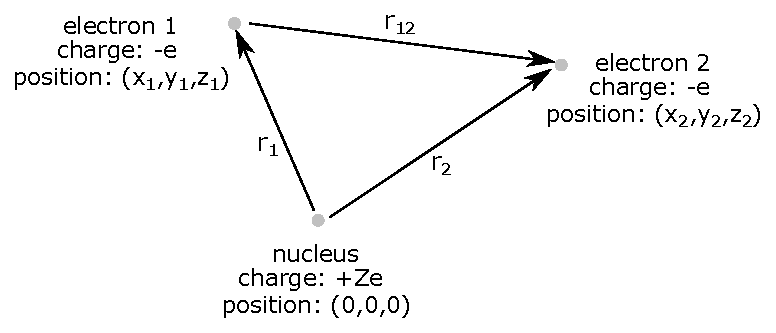
\includegraphics[width=0.5\textwidth]{includes/the-He-atom-FIGURES/He-atom}}
			%\end{minipage}
		
			\begin{parts}
				\part Assuming the nucleus is fixed in place (i.e. can't move), what is the \emph{kinetic} energy for the helium-like atom?  (You may use the $\nabla^2$ notation for the Laplacian(s); just put appropriate subscript(s) on it to indicate which set(s) of coordinates it refers to.)
				
					\begin{solution}[1.75in]
					\end{solution}				
				
				\part What is the \emph{potential} energy for this system?  Remember that the electrostatic energy of interaction between particles of charge $Q_1$ and $Q_2$ separated by distance $r$ is $\frac{Q_1Q_2}{4\pi\epsilon_0 r}$.
				
					\begin{solution}[1.75in]
					\end{solution}
				
				\part What is the \emph{Hamiltonian} for this system?
				
					\begin{solution}[1.5in]
					\end{solution}
				
				\contdnewpg
				\part The Hamiltonian you wrote (or should have written!) in part (c) is not separable.  Why? Which term causes the problem?
				
					\begin{solution}[2in]
					\end{solution}
				
				\part If you could ignore the ``problem'' term, what form do you think the wavefunction would take? You may write your answer out in words if you'd like; we'll formalize the notation together as a class.
				
					\begin{solution}[2.5in]
					\end{solution}
				
				\part If you calculated an expectation value for the energy using this simplified wavefunction and the full Hamiltonian, do you think the answer would over- or under-estimate the true ground-state energy?  Why?
				
					\begin{solution}[2.25in]
					\end{solution}
			\end{parts}
	\end{questions}
	
\stophere
\section*{The Variational Principle\sectionmark{The Variational Principle}}

	In this set of exercises, we'll consider the value of the expectation value of the energy for an arbitrary state.  For these exercises, assume that the $\{\ket{n}\}$ are energy eigenstates, with $\hat H \ket{n} = E_n \ket{n}$.
	
\begin{questions}
	\question Suppose we pick an arbitrary state $\ket{\Psi_t} = \sum_n c_n \ket{n}$.
	
		\begin{parts}
			\part What is the expectation value of the energy, $E_t$, for this state?
			
				\begin{solution}[3in]
				\end{solution}
			
			\part Assuming that $E_0 < E_1 < E_2 < \dots$ (e.g. the energies increase as $n$ increases), what must be true about the relationship between $E_t$ and $E_0$?  Fill in the correct inequality symbol (e.g $=$, $>$, $\geq$, $<$, $\leq$) to express your answer mathematically.
			
				\begin{equation*}
					E_t \,\, \answerbox{30}\,\,  E_0
				\end{equation*}
				
				\vspace{0.1in}
			\part If we knew that $\ket{\Psi_t}$ were \emph{orthogonal} to $\ket{0}$, what would have to be true about $c_0$?  What energy is the lower bound on $E_t$ in this case?
			
				\begin{solution}[2.5in]
				\end{solution}
		\end{parts} 
		\contdnewpg
		
	\question With the relationships from the previous page in mind, we can revisit the helium atom.
	
		\begin{parts}
			\part Suppose we took the same wavefunction that we guessed earlier, but now treat the charge on the nucleus as a \emph{variable} rather than a constant - let's call it $Z'$ rather than $Z$.
			
				Propose a procedure that you could use to find the value of $Z'$ that gives the ``best'' possible solution for the ground state energy of the helium atom.
				
				\begin{solution}[4in]
				\end{solution}
				
			\part Do you think the optimized value of $Z'$ will be greater than or less than the ``true'' value of $Z$?  Why?  
			
			(\emph{You should think about this question in pureley chemical terms - no math or quantum needed here.  Hint: what phenomenon do we talk about when we describe e.g. why some protons have greater chemical shifts in NMR than others?})
		\end{parts}
	
\end{questions}
%%%%%%%%%%%%%%%%%%%%%%%%%%%%%%%%%%%%%%%%%
%
% (c) 2018 by Jennifer Laaser
%
% This work is licensed under the Creative Commons Attribution-NonCommercial-ShareAlike 4.0 International License. To view a copy of this license, visit http://creativecommons.org/licenses/by-nc-sa/4.0/ or send a letter to Creative Commons, PO Box 1866, Mountain View, CA 94042, USA.
%
% The current source for these materials is accessible on Github: https://github.com/jlaaser/quantum-exercises
%
%%%%%%%%%%%%%%%%%%%%%%%%%%%%%%%%%%%%%%%%%

\section*{Symmetry with Respect to Exchange\sectionmark{Exercise: Exchange Symmetry}}

	\begin{questions}
	
		\question The permutation operator, $\hat P_{12}$, swaps particles one and 2, e.g. $\hat P_{12} \psi(q_1,q_2) = \psi(q_2,q_1)$.
		
			\begin{parts}
				\part If we apply the permutation operator twice, what should we get? In other words, what is $\hat P_{12}^2 \psi(q_1,q_2)$?
				
					\begin{solution}[1.5in]
					\end{solution}
				
				\part If particles 1 and 2 are indistinguishable, then swapping them should give the same state, up to a constant.  That is, $\psi(q_2,q_1) = c\psi(q_1,q_2)$.
				
				Convince yourself that this means that $\hat P_{12}^2\psi(q_1,q_2) = c^2 \psi(q_1,q_2)$.  In conjunction with your answer to part (a), what does this tell you about the value of $c$?
				
					\begin{solution}[2in]
					\end{solution}
				
				\part Suppose $c=-1$.  What happens if the two particles are at the same spatial coordinates, i.e. $q_1=q_2$?  \emph{(Hint: start with $\psi(q_1,q_1) = -\psi(q_1,q_1)$ and solve for $\psi(q_1,q_1)$).}
				
					\begin{solution}[2.5in]
					\end{solution}
				
			\end{parts}
			
		\contdnewpg
		
		\question When $c=1$, we say that the wavefunction is \emph{symmetric} with respect to exchange, while when $c=-1$, we say it is \emph{antisymmetric} with respect to exchange.%Before we learned about spin, we wrote the ground state of the helium atom as $\psi(1,2) = 1s(1)1s(2)$.
		
			With this in mind, let's consider the ground state of the helium atom, this time including spin:
			
			\begin{parts}
			
				\part One way we could incorporate spin is simply to multiply the spatial wavefunction $1s(1)1s(2)$ by spin functions $\alpha(1)$, $\beta(2)$, etc.  If we do this, four possible descriptions of helium's ground state are:
				
					\begin{enumerate}[itemsep=12pt,topsep=12pt]
						\item $1s(1)\alpha(1)1s(2)\alpha(2)$
						\item $1s(1)\alpha(1)1s(2)\beta(2)$
						\item $1s(1)\beta(1)1s(2)\alpha(2)$
						\item $1s(1)\beta(1)1s(2)\beta(2)$
					\end{enumerate}
					
					%\vspace{6pt}
					In the space to the right, above, identify each of these wavefunctions as symmetric with respect to exchange of electrons 1 and 2, antisymmetric with respect to exchange, or neither.
					
					\vspace{12pt}
				\part Another way we could construct the ground state of the helium atom is using the determinant
					\begin{equation*}
						\psi(1,2) = \frac{1}{\sqrt{2}}\begin{vmatrix}1s(1)\alpha(1) & 1s(1)\beta(1) \\ 1s(2)\alpha(2) & 1s(2)\beta(2)\end{vmatrix}
					\end{equation*}
					Is this wavefunction symmetric or antisymmetric with respect to exchange?
					
					\emph{Hint: you can do this by multiplying the determinant out, but there is also a more elegant way to get to the answer - what happens to the determinant of a matrix if you swap two rows or two columns?}
				
			\end{parts}
	
\end{questions}

%%%%%%%%%%%%%%%%%%%%%%%%%%%%%%%%%%%%%%%%%
%
% (c) 2018 by Jennifer Laaser
%
% This work is licensed under the Creative Commons Attribution-NonCommercial-ShareAlike 4.0 International License. To view a copy of this license, visit http://creativecommons.org/licenses/by-nc-sa/4.0/ or send a letter to Creative Commons, PO Box 1866, Mountain View, CA 94042, USA.
%
% The current source for these materials is accessible on Github: https://github.com/jlaaser/quantum-exercises
%
%%%%%%%%%%%%%%%%%%%%%%%%%%%%%%%%%%%%%%%%%

\section*{The Effective Potential in the Hartree Method\sectionmark{Exercise: Hartree Method Effective Potential}}
	
	In this exercise, we'll think about the physical meaning of the effective potential in the Hartree Method.

	\begin{questions}
	
		\question Consider an electron with wavefunction $\phi(1)\equiv \phi(\vec{r_1})$:
			
			\begin{parts}
				\part What is the \emph{probability density} for this electron?
				
					\begin{solution}[2.25in]
					\end{solution}
				
				\part What is the probability of finding the electron in a specific volume element $d\tau_1$ near position $\vec{r_1}$?
				
					\begin{solution}[2.25in]
					\end{solution}
				
				\part On average, how much charge is in this volume element $d\tau_1$?  (Remember that a single electron has charge $e$.)
				
					\begin{solution}[2in]
					\end{solution}
				
				\contdnewpg
				
				\part Suppose there is another electron (let's call it electron 2) at position $\vec{r_2}$.  What is the potential energy for the interaction between electron 2 and the little piece of electron 1's charge in volume element $d\tau_1$ near position $\vec{r_1}$?
				
					\begin{solution}[2in]
					\end{solution}
				\part What is the total potential energy for electron 2 at position $\vec{r_2}$ interacting with electron 1 (i.e. what do we get if we integrate over all possible positions of electron 1)?
				
					\begin{solution}[2in]
					\end{solution}
				
				\part Compare your answer to part (e) with the following expression for $V_{eff}$, the effective potential in the Hartree method:
			\begin{equation*}
				V_{eff}(\vec{r_2}) = \int d\tau_1 \, \phi^*(1)\frac{e^2}{4\pi \epsilon_0 r_{12}} \phi(1)
			\end{equation*}
			Explain, in your own words, why we might say that $V_{eff}$ is the potential that electron 2 ``sees'' when it interacts only with the average charge distribution of electron 1.
				
					\begin{solution}[2.25in]
					\end{solution}
			\end{parts}
	
\end{questions}

\stophere
%%%%%%%%%%%%%%%%%%%%%%%%%%%%%%%%%%%%%%%%%
%
% (c) 2018 by Jennifer Laaser
%
% This work is licensed under the Creative Commons Attribution-NonCommercial-ShareAlike 4.0 International License. To view a copy of this license, visit http://creativecommons.org/licenses/by-nc-sa/4.0/ or send a letter to Creative Commons, PO Box 1866, Mountain View, CA 94042, USA.
%
% The current source for these materials is accessible on Github: https://github.com/jlaaser/quantum-exercises
%
%%%%%%%%%%%%%%%%%%%%%%%%%%%%%%%%%%%%%%%%%

\section*{First-Order Perturbation Theory\sectionmark{Exercise: First-Order Perturbation Theory}}

	For a perturbed Hamiltonian, $\hat H = \hat H^{(0)} + \lambda \hat H^{(1)}$, we can write the full solutions to the Schr\"odinger equation as expansions of the form
	\begin{align*}
		E_n = E_n^{(0)} + \lambda E_n^{(1)} + \lambda^2 E_n^{(2)} + \dots & & \ket{n} = \ket{n^{(0)}} + \lambda\ket{n^{(1)}} + \lambda^2 \ket{n^{(2)}} + \dots
	\end{align*}
	In this set of exercises, we'll consider a simplified version of this problem where only keep terms that are zeroth and first order in $\lambda$, e.g.
	\begin{align*}
		E_n \approx E_n^{(0)} + \lambda E_n^{(1)} & & \ket{n} \approx \ket{n^{(0)}} + \lambda\ket{n^{(1)}}
	\end{align*}

	\begin{questions}
	
		\question 
		\begin{parts}
			\part Substitute the above expressions for $\hat H$, $\ket n$, and $E_n$ into the Schr\"odinger equation ($\hat H \ket{n} = E_n\ket{n}$) and multiply out both sides of the resulting equation.
			
				\begin{solution}[3in]
				\end{solution}
		
			\part If $\lambda=0$, what equation results?  Discuss, in your group, why this makes physical sense.
			
				\begin{solution}[1.25in]
				\end{solution}
		
			\part When $\lambda \neq 0$, the only way for the equation to hold is if the term(s) on the left side that scale as $\lambda^a$ are equal to the term(s) on the right side that scale as $\lambda^a$.  What equation results if you require this to be true for $a=1$, i.e. the terms that scale as $\lambda$?
			
		\end{parts}
		
		\newpage
		\question If we overlap both sides of this equation with $\bra{n^{(0)}}$, we obtain
				\begin{align*}
					\underbrace{\braket{n^{(0)}|H^{(1)}|n^{(0)}}}_A + \underbrace{\braket{n^{(0)}|\hat H ^{(0)}|n^{(1)}}}_B = \underbrace{\braket{n^{(0)}|E_n^{(1)}|n^{(0)}}}_C + \underbrace{\braket{n^{(0)}|E_n^{(0)}|n^{(1)}}}_D
				\end{align*}
		\begin{parts}
			\part Term $C$ is easy to simplify, as long as we require that the zeroth-order states (the $\ket{n^{(0)}}$) are orthonormal.  If this is true, what is term $C$ equal to?
			
				\begin{solution}[1.25in]
				\end{solution}
			
			\part We usually also require that the first-order corrections are orthogonal to the zeroth-order states, e.g. $\braket{n^{(0)}|n^{(1)}}=0$ (this requirement is called \emph{intermediate} normalization). If this is true, how can you simplify term $D$?
			
				\begin{solution}[1.25in]
				\end{solution}
			
			\part Term $B$ is trickier, but if we remember that $\hat H^{(0)}$ is Hermitian, we can rewrite it as $\braket{n^{(0)}|\hat H ^{(0)}|n^{(1)}} = \braket{n^{(1)}|\hat H ^{(0)}|n^{(0)}}^*$. Using this trick, and remembering that $\hat H ^{(0)}\ket{n^{(0)}} = E_n^{(0)}\ket{n^{(0)}}$, how can you simplify this term?
			
				\begin{solution}[1.75in]
				\end{solution}
			
			\part Substitute your answers to parts a-c in to the equation at the top of the page. In your group, discuss what the resulting equation tells you about the relationship between the zeroth-order states and the first-order corrections to the energy and Hamiltonian.
			
				\begin{solution}[1.25in]
				\end{solution}
		\end{parts}
	
	\end{questions}
	
\stophere
%%%%%%%%%%%%%%%%%%%%%%%%%%%%%%%%%%%%%%%%%
%
% (c) 2018 by Jennifer Laaser
%
% This work is licensed under the Creative Commons Attribution-NonCommercial-ShareAlike 4.0 International License. To view a copy of this license, visit http://creativecommons.org/licenses/by-nc-sa/4.0/ or send a letter to Creative Commons, PO Box 1866, Mountain View, CA 94042, USA.
%
% The current source for these materials is accessible on Github: https://github.com/jlaaser/quantum-exercises
%
%%%%%%%%%%%%%%%%%%%%%%%%%%%%%%%%%%%%%%%%%

\section*{Degenerate Perturbation Theory\sectionmark{Exercise: Degenerate Perturbation Theory}}

	As discussed in class, the approach described in the previous exercise fails when any of the zeroth-order states are degenerate. In this exercise, we'll consider how to transform our basis set to solve this problem.

	\begin{questions}
	
		\question 
		\begin{parts}
			\part Suppose the states $\{\ket{i^{(0)}}\}$ are degenerate, i.e. $\hat H^{(0)}\ket{i^{(0)}} = E \ket{i^{(0)}}$ for all of the states with different $i$.
			Calculate $H^{(0)}\ket{n^{(0)}}$, where $\ket{n^{(0)}}$ is a linear combination of these states, e.g. $\ket{n^{(0)}} = \sum_i c_{in}\ket{i^{(0)}}$. 
			
				\begin{solution}[5in]
				\end{solution}
			
			\part Explain why your result means that we can change our basis to any linear combination of the degenerate eigenfunctions without changing the result of our calculation.
			
				\begin{solution}[1.5in]
				\end{solution}
			
		\end{parts}
		\newpage
		
		\question An ``easy'' solution to our degeneracy problem is to require that the numerator, $\braket{m^{(0)}|\hat H^{(1)}|n^{(0)}}$, equals zero whenever $n\neq m$.
		
			\begin{parts}
			
				\part Substitute $\ket{n^{(0)}} = \sum_i c_{in}\ket{i^{(0)}}$ and $\ket{m^{(0)}} = \sum_j c_{jm}\ket{j^{(0)}}$ into $\braket{m^{(0)}|\hat H^{(1)}|n^{(0)}}$ and simplify the expression until it is in terms of $c_{in}$, $c_{jm}$, and $H_{ji}^{(1)}$ (where $H_{ji}^{(1)} = \braket{j^{(0)}|\hat H^{(1)}|i^{(0)}}$ are the matrix elements of the perturbation Hamiltonian).
				
					\begin{solution}[3.5in]
					\end{solution}
				
				\part Remembering that $c_{jm}^* = (\umat{c}^\dag)_{mj}$, how can you rewrite this expression using a matrix product?
				
					\begin{solution}[2in]
					\end{solution}
				
				\part In order for $\braket{m^{(0)}|\hat H^{(1)}|n^{(0)}}$ to be nonzero when $n=m$ but zero otherwise, the resulting matrix must be a \emph{diagonal} matrix.
				
					Explain, in words, what this means about the matrix $\umat{c}$ containing the coefficients $c_{in}$.
				
					\begin{solution}[1in]
					\end{solution}
			
			\end{parts}
	
	\end{questions}

	
\end{document}
